\documentclass[a4paper]{article}

\usepackage[utf8]{inputenc}

\usepackage{url}
\usepackage[]{hyperref}

\usepackage{caption}

\usepackage{listings}

\usepackage{color}

% *** GRAPHICS RELATED PACKAGES ***
%\usepackage[pdftex]{graphicx}
\usepackage{graphicx}
%\usepackage[dvips]{graphicx}
% to place figures on a fixed position
\usepackage{float}

\usepackage[margin=1in]{geometry}

\title{OpenFlow \& Mininet – Docker}
\author{}
\date{}


\begin{document}

\maketitle

\tableofcontents

\section{Linux containers}
A Linux konténerek (LXC) operációs rendszer szintű virtualizált környezetet nyújtanak, amelyben izolált Linux rendszerek (konténerek) futtathatók a Linux hosztgépen. Az operációs rendszer szintű virtualizált környezetet tekinthetjük a virtuális gépek (Virtaul Machine – VM) könnyített verziójának. Mivel jobb ez mint egy virtuális gép? Kevesebb helyet foglal egy virtuális vendégrendszer, gyors a létrehozása és működése, kevesebb a helyfoglalás – szemben a teljes virtuális megoldásokkal. A konténerek ahelyett, hogy a teljes hardveres környezetet emulálnának, egy közös, megosztott operációs rendszer magot (kernel) használnak, ezáltal hatékonyabb futásra képesek, mint a VM technológiák megoldásai.

Másik megközelítésben: ``chroot on streoids" jelzővel is illetik. A chroot művelet egy parancsot vagy az interaktív shellt a paraméterben megadott speciális gyökérkönyvtárral futtatja. A futó folyamat mintegy be van zárva ebbe a könyvtárba, nem tudja az azon kívüli fájlokat elérni. Ezzel egy kisebb rendszert hozhatunk létre a nagyobbik rendszeren belül. 

\begin{figure}[H]
    \centering
    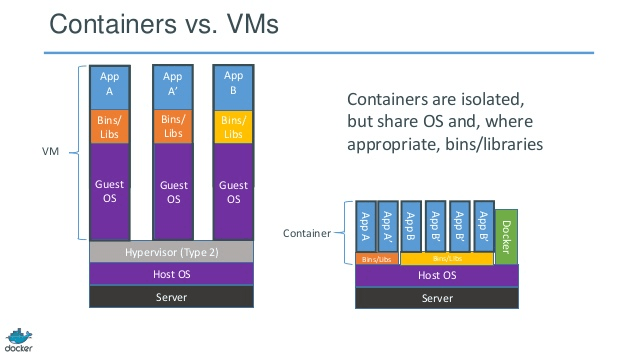
\includegraphics[width=0.9\textwidth]{figures/container_vs_vm.png}
    \caption{Containers vs. VMs}
    \label{fig:containers}
\end{figure}

A Linux kernel control groups (cgroups) funkciója tudja biztosítani az erőforrások felosztását és proiritizálását, anélkül, hogy virtuális gépeket kellene indítani, valamint a névterek (namespaces) segítségével lehet leválasztani az egyes alkalmazások számára, hogy mit láthatnak az operációs rendszer által nyújtott környezetből, úgymint folyamatokat, fájlrendszereket, felhasználói azonosítókat és a hálózati kapcsolatokat. Ennek eredményeként egy saját egy futtatókörnyezetet hozunk létre alkalmazásunk számára, amely a többi konténertől és a hosztgéptől is leválasztott módon működik. Az alkalmazás mellé annak környezetét és függőségeit (programcsomagok, függvénykönyvtárak, konfigurációs fájlok, stb.) is a konténerbe ágyazhatjuk, ezáltal könnyen hordozható, leállítható és újraindítható egységet kapunk. Például létrehozhatunk egy konténert a webszerverünknek, egyet az adatbázisunknak, egyet az üzenetkezelőnek (message queue), vagy épp csomagolhatjuk őket egybe is, stb. ezzel moduláris alkalmazás architektúrát kialakítva. Ha saját fejlesztésű szoftvert konténer(ek)be csomagolunk, akkor az így kiadott szoftver biztosan futni fog másik hosztgépen is, legyen az egy másik fejlesztői vagy tesztelői PC, vagy akár az alkalmazás szerver vagy virtuális gép, amire a kész alkalmazást telepíteni fogjuk, vagyis nagyon felxibilis hordozhatóság szempontjából. Ami pedig egy Linux gépen futtatható, azt be lehet csomagolni egy Linux konténerbe is. A konténerek egy új, könnyebb módot adnak a fejlesztési folyamatban az alkalmazások kódolása, fordítása, telepítése és futtatása számára, és egyszerűen telepíthetők akár a felhő szolgáltatók gépeire is.

\section{Docker}

A Docker egy nyílt platformot nyújt a konténerek könnyű kezeléséhez, amellyel elosztott alkalmazások fejleszthetünk és futtathatunk, könnyű hordozhatóság mellet. Egy olyan közös eszközhalmazt ad a programozók, fejlesztői csapatok (development) és üzemeltetők (operations) kezébe amellyel kihasználhatják az elosztott és hálózati alkalmazások előnyeit. A Docker futtató környezete daemonként fut a háttérben és kezeli a konténereket, image-eket és a létrehozási folyamatokat.

A Docker célja az LXC használatának egyszerűsítése, kényelmessé tétele volt, emellett lehetővé teszi, hogy a konténerek különböző Linux rendszerek közt is hordozhatóak legyenek, vagyis elfedi az LXC rendszerspecifikus részeit. Kezdetben a Docker LXC-t használt, mára a Dockernek saját konténer formátuma van. Egy fontos különbség: LXC konténerekben van init, így több folyamatot is futtathatunk, míg Docker konténerekben nincs, így csak egyet. (A különbségeket részletesebben lásd itt: https://www.flockport.com/lxc-vs-docker/)

A Docker architektúrája kliens-szerver modellre épül. A Docker kliens által kiadott parancsokat a Docker daemon (docker engine, szerver) hajtja végre. A felhasználó a Docker daemonnal nincs közvetlen kapcsolatban, csak a kliensen keresztül, ez maga a ``docker" program, ami a felhasználói felületet adja. A kliens és a daemon futhat ugyanazon a számítógépen, vagy a kliens kapcsolódhat távoli daemonhoz. A kommunikáció socketen vagy RESTful API-n keresztül történik.

\begin{figure}[H]
    \centering
    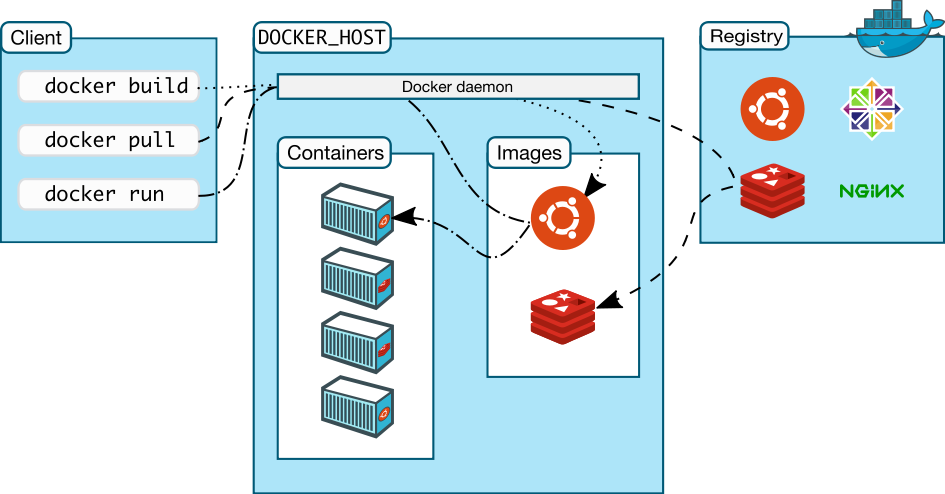
\includegraphics[width=0.9\textwidth]{figures/docker_arch.png}
    \caption{Docker components and architecture}
    \label{fig:arch}
\end{figure}

A docker használatához szükség van egy képfájlra (image) az adott operációs rendszerből. A képfájl egy írásvédett sablon, aminek segítségével a konténerek elindíthatók. A konténer futtatásakor ez kiegészül egy felső írható fájlrendszer réteggel, amelyben a saját alkalmazásunk futhat. A képfájl tulajdonképpen egy előtelepített rendszer, felépítése aufs vagy btrfs rétegek összességéből áll (Union File System), és verziókezelt. Kiindulásul van egy alap képfájl (base image), pl. ubuntu vagy debian, és az efelett elhelyezkedő fájlrendszer rétegetek egyesülnek a végleges képfájllá. Bármely képfájlra, nem csak az alapra, további rétegeket lehet építeni, így kiegészítve, változtatva azon a saját igényeink szerint. Képfájlok elkészíthetők saját magunk által vagy mások által előállított képfájlok letölthetők a docker úgynevezett Docker Hub webhelyéről. Ez egy központi tároló, de lehet saját, magáncélút is kialakítani. Az egyedileg elkészített képfájlok feltölthetők, megoszthatók a közösséggel.

\begin{figure}[H]
    \centering
    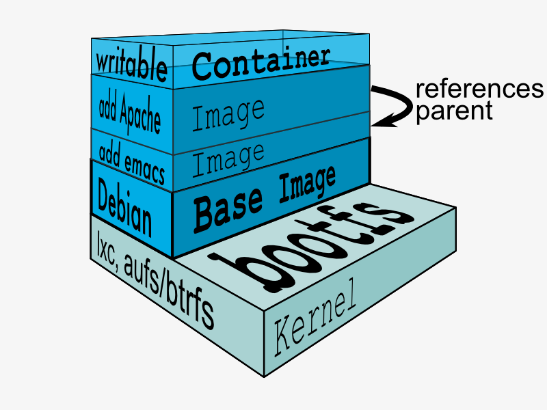
\includegraphics[width=0.9\textwidth]{figures/docker_layers.png}
    \caption{Docker layers}
    \label{fig:layers}
\end{figure}

A konténer egy adott képfájl futó (vagy futott) példánya. Egy képfájlból egyszerre több konténer példány is futhat.

Docker képfájlok kialakítása, továbbfejlesztése két módon lehetséges: egyrészt a futó konténerbe belépve manuálisan installálva és konfigurálva, majd az előállt képfájlt elmentve, másrészt ún. Dockerfile segítségével, amely saját parancsformátummal rendelkezik és szkriptszerűen leírhatók a telepítendő komponensek.

\section{Further Reading}



\begin{itemize}
    \item Docker áttekintés: \url{https://docs.docker.com/engine/docker-overview/}
    \item Docker bevezetés: \url{https://docs.docker.com/get-started/} Part 1. and 2.!
\end{itemize}


\appendix

\section{Entry quiz sample questions}

\begin{enumerate}
  \item Mi a különbség a virtuális gépek és a linux konténerek között?
  \item Milyen linux funkciók teszik lehetővé a konténerek megvalósítását?
  \item Hogyan viszonyulnak egymáshoz a Docker képfájlok (image) és konténerek (container)?
  \item Hogyan használhatók a Docker képfájlok (image), ki hozhatja létre, hogyan lehet hozzáférni?
  \item Miként lehet kiegészíteni, továbbfejleszteni egy Docker képfájlt (image)?
  \item Mi a funkciója az interaktív és a dameon módnak?
  \item Mi a különbség a docker run és docker start parancsok között?
  \item Hogyan lehet a konténer hálózati portjait a hoszt gépre leképezni? 
\end{enumerate}

\section{Lab exercises}

\subsection{Lab environment \& introduction}
\subsubsection{List of important commands}

\subsection{Task 1.}
\subsubsection{Application containers}
\subsubsection{Interconnecting two containers}
\subsubsection{Web content and database upload}
\subsection{Task 2.}
\subsection{Task 3.}

\end{document}